\documentclass{article}

\usepackage{amsmath, amssymb}
\usepackage{listings}
\usepackage{float}
\usepackage{tikz}
\usetikzlibrary{automata, arrows.meta, positioning}
\usepackage{caption}
\usepackage{subcaption}

\author{Xiaoyue Chen}
\title{1DV517\\Assignment 2 report}

\begin{document}
\maketitle

\section{}
\subsection{}
\begin{align*}
	G =      & \langle V, \Sigma, R, S \rangle             \\
	\Sigma = & \{ a, b \}                                  \\
	V =      & \{ S \}                                     \\
	R =      & \{ S \rightarrow abS | bS | a | \epsilon \}
\end{align*}

\subsection{}
\begin{align*}
	G =      & \langle V, \Sigma, R, S \rangle              \\
	\Sigma = & \{ a, b, c \}                                \\
	V =      & \{ S \}                                      \\
	R =      & \{ S \rightarrow aSb | aS | cS | \epsilon \}
\end{align*}

\subsection{}
\begin{align*}
	G =      & \langle V, \Sigma, R, S \rangle    \\
	\Sigma = & \{ a, b, c \}                      \\
	V =      & \{ S, A, B, C, D \}                \\
	R =      & \{                                 \\
	         & S \rightarrow aAa | bBb | cCc | D, \\
	         & A \rightarrow DAD | a,             \\
	         & B \rightarrow DBD | b,             \\
	         & C \rightarrow DCD | c,             \\
	         & D \rightarrow a | b | c            \\
	\}
\end{align*}

\subsection{}
\begin{align*}
	G =      & \langle V, \Sigma, R, S \rangle           \\
	\Sigma = & \{ a, b, c \}                             \\
	V =      & \{ S, A, B, C \}                          \\
	R =      & \{                                        \\
	         & S \rightarrow AB,                         \\
	         & A \rightarrow CAC | CA | C,               \\
	         & B \rightarrow aBa | bBb | cBc | \epsilon, \\
	         & C \rightarrow a | b | c                   \\
	\}
\end{align*}

\section{}
The CNF can append an arbitrary number of $0$s to the right
of
a string by applying rule $S \rightarrow S0$. It can also append an
arbitrary number of $0$s or $01$s to the
left of a string by applying rule $S \rightarrow 1S$ and
$S \rightarrow 01S$ respectively. Hence we could express this language with
$(1|01)^* 0^*$.

The $(1|01)^*$ part of the regular expression could not accept
$2$ continuous $0$s, they have to be
accepted by the $0^*$ part. However, there is nothing to
accept the last $1$ in $001$ in the regular
expression. Hence this language contains no substring 001.

\section{}

\begin{figure}[H]
	\centering
	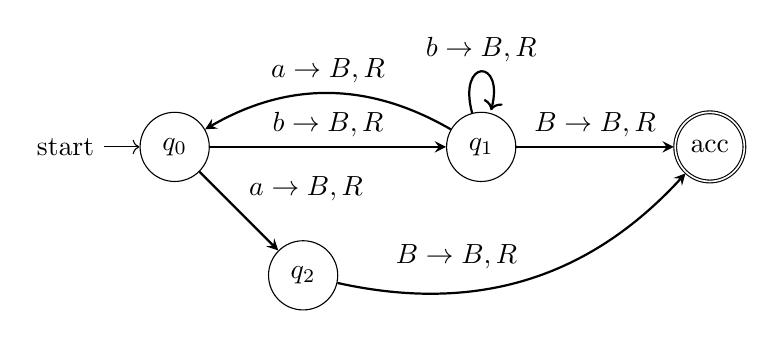
\begin{tikzpicture} [auto]
		\node (q0) [state, initial] {$q_0$};
		\node (q1) [state, right = 3cm of q0] {$q_1$};
		\node (q2) [state, below right = of q0] {$q_2$};
		\node (acc) [state, accepting, right = 2cm of q1] {acc};
		\path [-stealth, thick]
		(q0) edge node {$b \rightarrow B, R$} (q1)
		(q0) edge node {$a \rightarrow B, R$} (q2)
		(q1) edge [loop above] node {$b \rightarrow B, R$} ()
		(q1) edge [bend right] node [above] {$a \rightarrow B, R$} (q0)
		(q1) edge node {$B \rightarrow B,R$} (acc)
		(q2) edge [bend right] node {$B \rightarrow B, R$} (acc)
		;
	\end{tikzpicture}
\end{figure}

$B$ means blank in the Turing machine above. Since the CFG
could only generate symbols from left to right, our Turing machine could
check the string from left to right to see if every step adhere to the CFG
rules.

The Turing machine reads the first symbol and check if it is an
$a$ or $b$. An $a$
means rule $S \rightarrow a$ is applied as the first step. It generates
only a terminal, so the machine expects a blank. Otherwise the machine will
reject the string. If the first symbol is a $b$, it means
$S \rightarrow bA$ is applied as the first step. Then the machine moves to
the right to read the second symbol and determine which of the
$A$ rules is applied in the same way.

The machine continues to move to the right and determine which rule is applied.
If it could not find any rule allowed at the state, it rejects the string. If a
blank is reached after applying a rule that generates only a terminal
($S \rightarrow a$ or $A \rightarrow \epsilon$), the machine accepts the
string.

\section{}
\subsection{}
Consider to derive the string $ac$ using the grammar. It
could result in 2 different parse trees:

\begin{figure}[H]
	\begin{subfigure}{.5\textwidth}
		\centering
		\begin{tikzpicture}[->]
			\node{$S$}
			child{node{$a$}}
			child{node{$S$}
					child{node{$A$}
							child{node{}}
						}
					child{node{$S$}
							child{node{}}
						}
					child{node{$c$}}
				}
			;
		\end{tikzpicture}
	\end{subfigure}%
	\begin{subfigure}{.5\textwidth}
		\centering
		\begin{tikzpicture}[->]
			\node{$S$}
			child{node{$A$}
					child{node{}}
				}
			child{node{$S$}
					child{node{$a$}}
					child{node{$S$}
							child{node{}}
						}
				}
			child{node{$c$}}
			;
		\end{tikzpicture}
	\end{subfigure}
\end{figure}

\subsection{}
The grammar is ambiguous because of indirect left-recursion. If we remove
rule $A$, we get
\begin{align*}
	S & \rightarrow  aS ~|~ bBSc ~|~ Sc ~|~ \epsilon \\
	B & \rightarrow bBSa ~|~ Sa
\end{align*}

After substituting $S$ in rule $B \rightarrow Sa$
\begin{align*}
	S & \rightarrow  aS ~|~ bBSc ~|~ Sc ~|~ \epsilon      \\
	B & \rightarrow bBSa ~|~ aSa ~|~ bBSca ~|~ SSca ~|~ a
\end{align*}

The rule $S \rightarrow Sc$ is left-recursive. Also, the rules
$B \rightarrow bBSa ~|~ bBSca$ require left factoring. Hence the grammar is ambiguous.

\subsection{}
After removing left-recursion
\begin{align*}
	S  & \rightarrow aS' ~|~ bBScS' ~|~ S' \\
	S' & \rightarrow cS' ~|~ \epsilon      \\
	B  & \rightarrow bBSa ~|~ Sa
\end{align*}

Removing $S$ in $B \rightarrow Sa$
\begin{align*}
	S  & \rightarrow aS' ~|~ bBScS' ~|~ S'             \\
	S' & \rightarrow cS' ~|~ \epsilon                  \\
	B  & \rightarrow bBSa ~|~ bBScS'a ~|~ aS'a ~|~ S'a
\end{align*}

Left-factorize $bBS$ in the rules for $B$
\begin{align*}
	S  & \rightarrow aS' ~|~ bBScS' ~|~ S'  \\
	S' & \rightarrow cS' ~|~ \epsilon       \\
	B  & \rightarrow bBSB' ~|~ aS'a ~|~ S'a \\
	B' & \rightarrow a ~|~ cS'a
\end{align*}

Above is the final unambiguous grammar.

\end{document}
